%------------------------------------------------
\begin{frame}
\frametitle{Equilibrium Exercises}
\hypertarget{vesti}{}
\begin{columns}[c] % The "c" option specifies centered vertical alignment while the "t" option is used for top vertical alignment

\column{.4\textwidth} % Left column and width

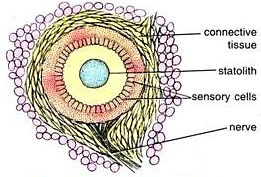
\includegraphics[width=\linewidth]{statolith.jpg}

The vestibularium is a  \structure{liquid filled organ} in the inner ear. It allows us to balance.
The statolith is like a tiny
\structure{ball that sinks} in the fluid.
\note{When a person is in a drunk state the viscosity of the liquid in the vestibularium increases due to dehydration, the statolith ball stays afloat and the person has therefore no sense of what's up and down.}
\pause

\column{.5\textwidth} % Left column and width
Being in equilibrium means a \structure{bringing our body in balance}, on many levels.

Inside as outside of the body, everything is \structure{in harmony and connected}, a harmony between the person and the surroundings, the universe gets created.

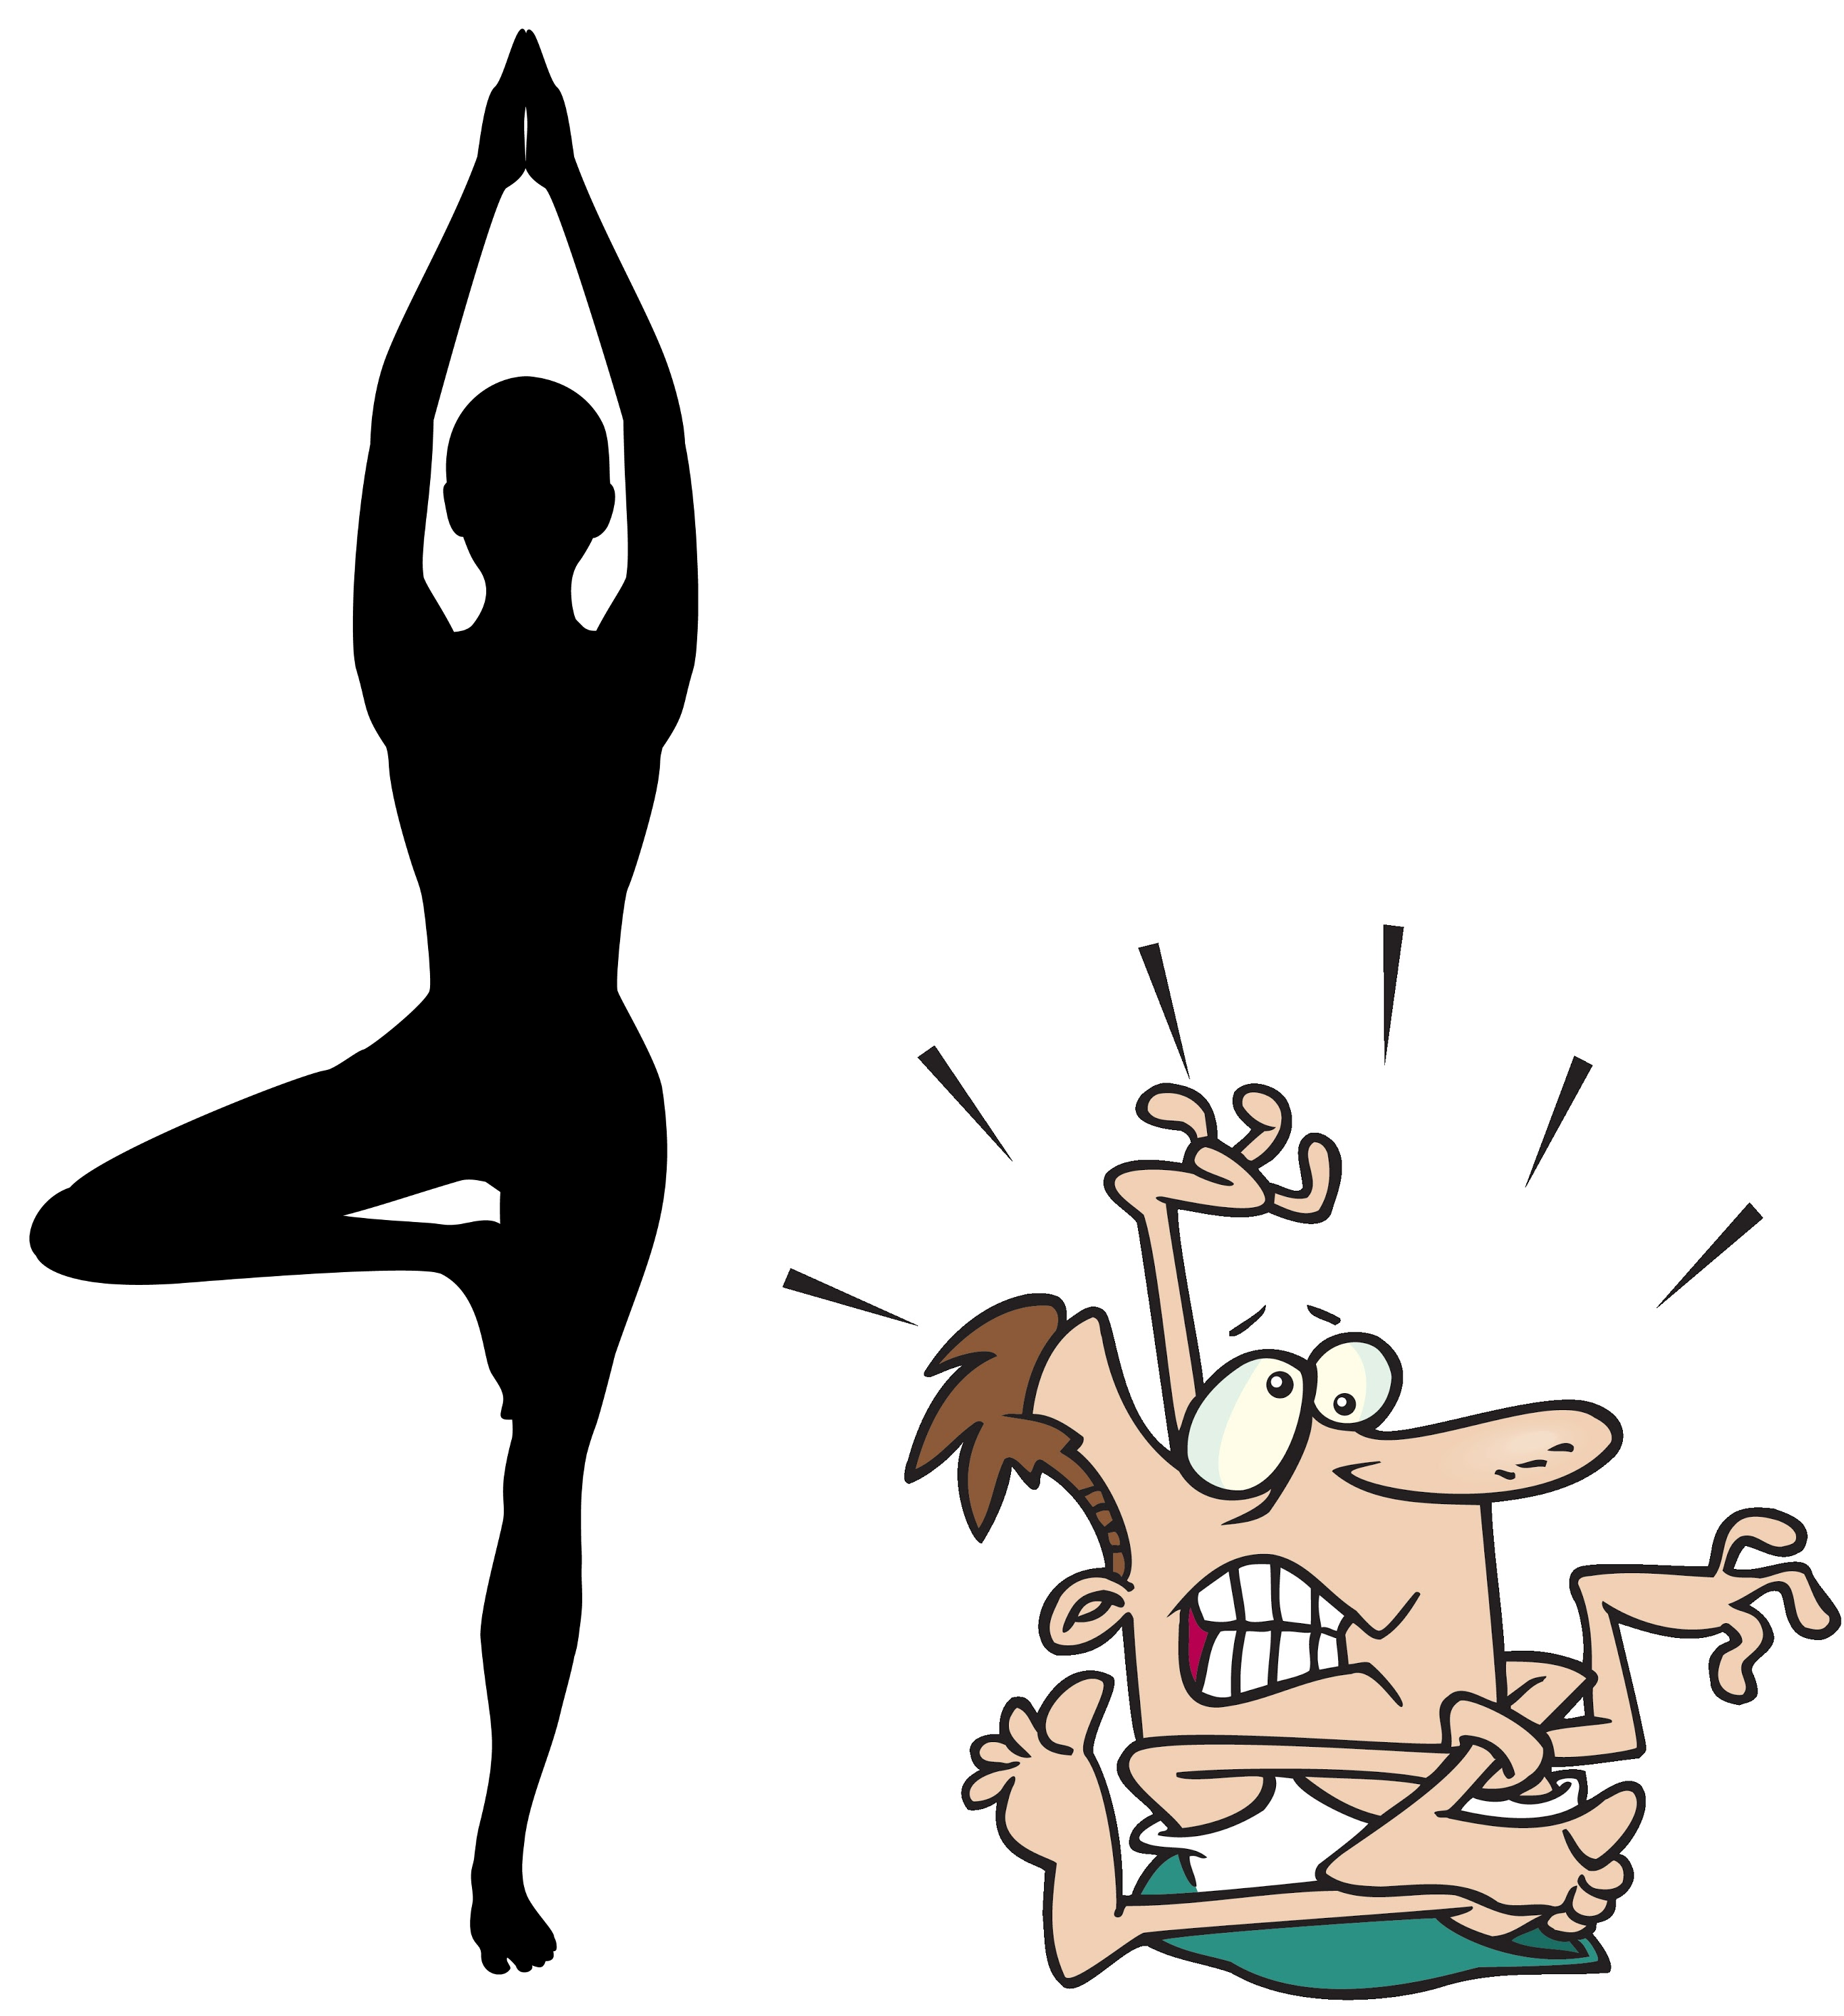
\includegraphics[width=0.6\linewidth]{yoga.png}

\end{columns}

\end{frame}
%------------------------------------------------
